\documentclass[conference]{IEEEtran}

\usepackage{amsmath}
\usepackage{array}
\usepackage{booktabs}
\usepackage{cite}
\usepackage{graphicx}
\usepackage[hidelinks]{hyperref}
\usepackage{tabularx}

\graphicspath{{../modeling/figures/}{../dashboard/screenshots/}{../eda/figures/}}

\newcolumntype{Y}{>{\raggedright\arraybackslash}X}
\newcolumntype{L}[1]{>{\raggedright\arraybackslash}p{#1}}

\begin{document}

\title{Explainable Grid-Time Traffic Incident Risk Prediction in Dubai}

\author{
\IEEEauthorblockN{Sparsh Aggarwal}
\IEEEauthorblockA{Department of Computer Science\\
BITS Pilani, Dubai Campus\\
Dubai, United Arab Emirates}
\and
\IEEEauthorblockN{Dr. Sujala D. Shetty}
\IEEEauthorblockA{Department of Computer Science\\
BITS Pilani, Dubai Campus\\
Dubai, United Arab Emirates}
}

\maketitle

\begin{abstract}
This paper presents an explainable machine-learning framework for non-recurrent traffic incident risk prediction in Dubai. The study uses 720,155 open Dubai Police incident records from 13 August 2018 to 1 June 2026. Arabic incident categories are translated and parsed, mixed coordinate order is corrected, and incident points are converted into H3 resolution-8 cells and 3-hour windows. The prediction target is binary: whether an inside-Dubai grid cell contains at least one incident in a given window. Models are trained with chronological splitting and evaluated on a full inside-Dubai grid rather than only on a sampled-negative table. The selected model is an XGBoost classifier using calendar features, historical-risk priors, same-cell lag features, and ring-1 neighboring-cell lag features. Neighboring lag features improve full-grid PR-AUC from 0.0967 to 0.0992 and F1-score from 0.1615 to 0.1645 compared with the same XGBoost setup without neighbor features. The model captures 10,416 incidents in the top-20 ranked cells per test window. Sigmoid calibration improves probability reliability for dashboard display, while SHAP and LIME are used to explain model behavior. The resulting dashboard demonstrates rolling replay with ranked Dubai risk zones and local explanation reasons.
\end{abstract}

\begin{IEEEkeywords}
Traffic incident prediction, explainable AI, H3 grid, XGBoost, SHAP, LIME, Dubai, road safety.
\end{IEEEkeywords}

\section{Introduction}

Non-recurrent traffic incidents include crashes, breakdowns, obstructions, roadwork reports, stalled vehicles, and other irregular events that reduce road capacity. They differ from regular congestion because they are not simply part of the daily peak pattern. In a dense road network such as Dubai, these events can affect safety, travel time, and traffic operations beyond the exact incident point.

Dubai road-safety studies have examined crash trends, causes, and hotspots \cite{aldah2010dubai,abdelfatah2015dubai,alsaleh2026dubaihotspots}. These studies establish the local road-safety context, but they do not fully address the question studied here: can open incident records be converted into an explainable grid-time prediction system for Dubai?

The contribution of this paper is a reproducible incident-only framework that moves from raw reported incident points to a model that ranks future grid/time windows inside a historical test period. The framework includes Arabic category parsing, coordinate correction, H3 grid construction, chronological model evaluation, full-grid test scoring, probability calibration, SHAP/LIME explanation, and a dashboard prototype. The work is a historical decision-support prototype. It does not claim live deployment, signal control, or causal explanation of incidents.

\section{Related work}

Traffic accident prediction has moved from descriptive aggregate analysis to spatiotemporal machine learning. Citywide accident-risk models show that historical incident patterns can be converted into region/time risk estimates \cite{ren2017citywide,zhou2020riskoracle}. Grid-based crash prediction supports the use of spatial cells when raw incident records are available as points \cite{kashifi2022grid}. Recent urban-risk studies also highlight sparsity, regionality, and spatial proximity as important challenges \cite{chen2024urbanrisk}. Review work on traffic accident prediction shows a broad shift toward machine-learning models, but also shows that datasets, evaluation designs, and deployment assumptions differ widely across studies \cite{behboudi2024review}.

Explainability has become important in traffic-safety modeling because black-box predictions are difficult to trust in operational settings. SHAP has been used to explain fatality and severity models \cite{rifat2024explainable,sufian2023severity}, while LIME provides a local model-agnostic alternative \cite{ribeiro2016lime}. This study applies these explanation methods to a different target: grid-time occurrence of reported non-recurrent incidents. SHAP and LIME are used to explain the trained model, not to identify physical causes of crashes or breakdowns.

\section{Data and preprocessing}

The primary data source is an open Dubai Police traffic incident dataset from Dubai's Data and Statistics portal. The frozen snapshot used in this study contains 720,155 incident-level rows and six raw fields: incident ID, incident time, Arabic incident category, two coordinate fields, and load timestamp. The incident period runs from 13 August 2018 to 1 June 2026.

The Arabic category field contains 233 unique strings. Each unique category was translated and parsed once, then joined back to the full dataset. The category string usually combines incident type and severity. Unknown or unspecified severity is kept as a separate class. It remains part of incident-occurrence prediction because the record still describes a real incident, but it is assigned severity weight zero for severity-weighted sums.

Coordinate validation was necessary because the raw file contains mixed coordinate order. The cleaning process keeps the raw coordinate fields and adds normalized longitude, latitude, and coordinate-status fields. After category and coordinate filtering, 717,615 rows are usable for map-based exploratory analysis. The cleaned point records are then assigned to H3 cells.

\section{Grid-time prediction formulation}

Each record is mapped to an H3 resolution-8 cell and a 3-hour time window. For each inside-Dubai H3 cell and each window, the label is one if at least one incident occurs and zero otherwise. This creates positive rows for observed incident cell/windows and negative rows for cell/windows without reported incidents.

The final inside-Dubai grid contains 1,305 H3 cells. The chronological split uses early windows for training, the next block for validation and calibration, and the last block for testing. The full-grid test set contains 4,463,100 candidate cell/windows, of which 108,224 are positive. This denominator is important because it reflects the real rarity of incidents across all evaluated cells and windows.

\section{Methodology}

The model features are restricted to information available before the target window. Calendar features include hour block, day of week, weekend flag, month, and year. Historical-risk features include train-period empirical risk for each cell, each hour block, and each cell-hour combination. Same-cell lag features count incidents in the previous 3 hours, 24 hours, and 7 days. Neighboring lag features aggregate the same type of recent history over H3 ring-1 cells inside Dubai.

Historical risk, Logistic Regression, Random Forest, and XGBoost are compared. XGBoost is used as the final model family because it handles non-linear tabular relationships and works well with mixed calendar, lag, and historical-risk features \cite{chen2016xgboost}. Models are trained with a sampled-negative training table for tractability, but validation and test evaluation use the full inside-Dubai grid.

The main metrics are ROC-AUC, PR-AUC, precision, recall, F1-score, and top-k hotspot metrics. PR-AUC is emphasized because positive cell/windows are rare \cite{saito2015prauc}. Top-k metrics rank all inside-Dubai cells for each test window and check how many actual incident cells or incidents are captured among the highest-risk cells.

\section{Results}

Table~\ref{tab:main_result} summarizes the main full-grid results. The historical-risk baseline is strong, which is expected because some zones and time blocks are repeatedly active. The initial XGBoost model improves over this baseline. Adding ring-1 neighboring lag features gives the best final result, with ROC-AUC 0.8120, PR-AUC 0.0992, recall 0.2720, precision 0.1179, and F1-score 0.1645.

\begin{table}[t]
\centering
\caption{Inside-Dubai full-grid test results}
\label{tab:main_result}
\scriptsize
\setlength{\tabcolsep}{3pt}
\begin{tabular}{L{0.37\columnwidth}rrrr}
\toprule
Model & ROC-AUC & PR-AUC & Recall & F1 \\
\midrule
Historical risk & 0.7990 & 0.0882 & 0.2679 & 0.1522 \\
XGBoost, no neighbor lags & 0.8067 & 0.0967 & 0.2630 & 0.1615 \\
XGBoost, neighbor lags & 0.8120 & 0.0992 & 0.2720 & 0.1645 \\
\bottomrule
\end{tabular}
\end{table}

Table~\ref{tab:topk_result} shows the top-20 hotspot result. The selected XGBoost model captures 9,138 positive cell/windows and 10,416 incidents in the top-20 ranked cells per test window. This result supports the use of the model as a hotspot-ranking tool. It should not be read as a claim that every individual incident can be predicted.

\begin{table}[t]
\centering
\caption{Top-20 hotspot ranking result}
\label{tab:topk_result}
\scriptsize
\setlength{\tabcolsep}{3pt}
\begin{tabular}{L{0.37\columnwidth}rrr}
\toprule
Model & Pos. cells & Incidents & Incident recall \\
\midrule
Historical risk & 8,847 & 10,043 & 0.0871 \\
XGBoost, no neighbor lags & 9,049 & 10,281 & 0.0892 \\
XGBoost, neighbor lags & 9,138 & 10,416 & 0.0903 \\
\bottomrule
\end{tabular}
\end{table}

Two additional model-improvement attempts were tested and rejected. A 70/30 hard-negative training sample reduced PR-AUC from 0.0992 to 0.0487 and F1-score from 0.1645 to 0.1015. A validation-selected tuned XGBoost configuration reduced test PR-AUC to 0.0976 and F1-score to 0.1620. The default neighbor-feature XGBoost model is therefore retained because it performs slightly better on the untouched test period and is easier to defend.

Sigmoid calibration is selected for dashboard probability display. It preserves PR-AUC and top-k ranking while reducing Brier score from 0.2127 to 0.0227 and equal-frequency expected calibration error from 0.3518 to 0.0013. Calibration is used for interpreting displayed risk values; it is not treated as a new ranking model.

\begin{figure}[t]
\centering
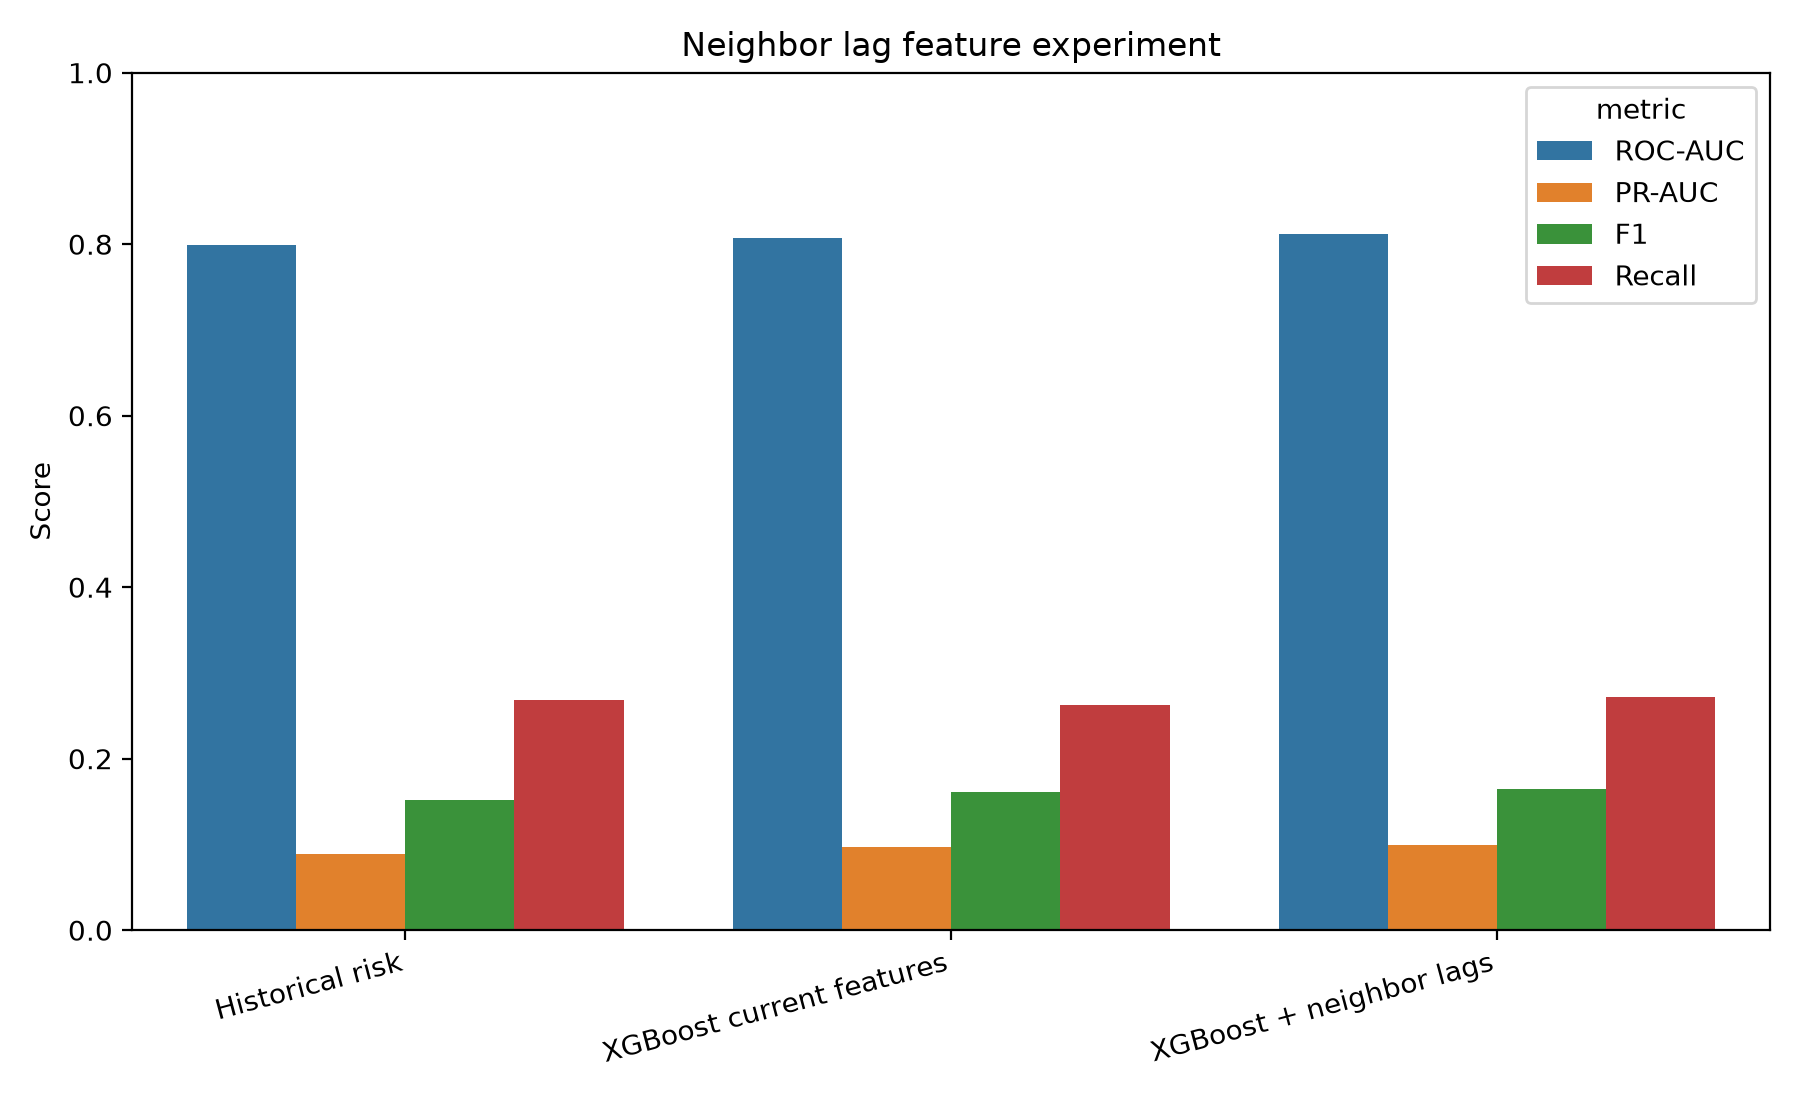
\includegraphics[width=\columnwidth]{neighbor_lag_feature_model_comparison.png}
\caption{Full-grid performance comparison for historical risk, XGBoost without neighbor lags, and XGBoost with neighbor lags.}
\label{fig:neighbor_model_comparison}
\end{figure}

\section{Explainability}

SHAP is used as the main explanation method for the selected XGBoost model \cite{lundberg2017shap}. The strongest grouped feature is historical cell-hour risk. Other important groups include year, historical cell risk, previous 7-day same-cell incident count, previous 7-day neighboring-cell incident count, weekend flag, and previous 24-hour neighboring-cell incident count.

\begin{figure}[t]
\centering
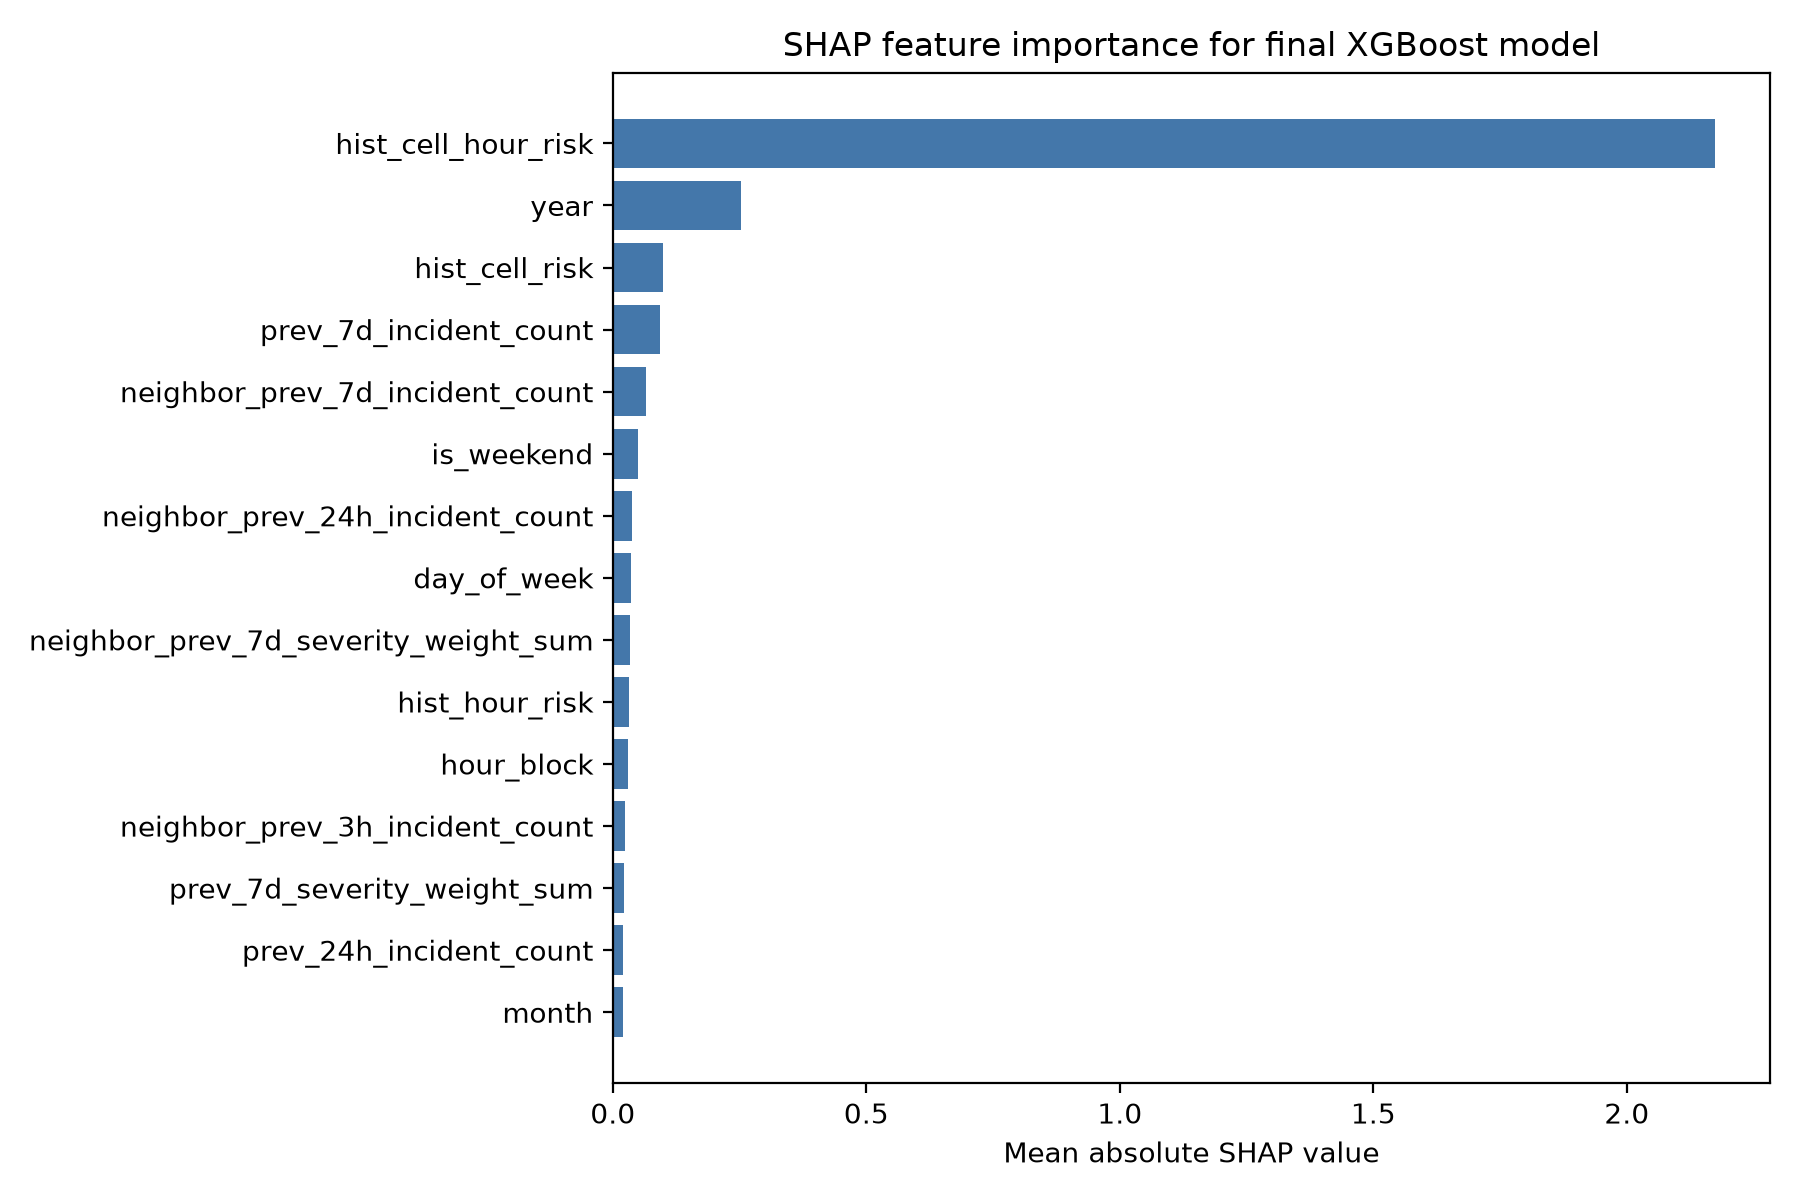
\includegraphics[width=\columnwidth]{shap_feature_importance_bar.png}
\caption{Grouped SHAP feature importance for the selected neighbor-feature XGBoost model.}
\label{fig:shap_importance}
\end{figure}

LIME is used as a supporting local comparison on selected cases. For high-risk true-positive and false-positive cases, both methods usually highlight historical cell-hour risk and recent same-cell or neighboring activity. For low-score false-negative and true-negative cases, low historical risk and little recent activity tend to push the model score down. These explanations describe how the trained model uses engineered features. They do not prove that those features caused the incident.

\section{Dashboard prototype}

The dashboard presents the model through rolling replay. It defaults to complete observed days before the data cutoff and displays the highest-ranked H3 cells on an English map. A zone-explanation view shows the selected cell, time window, calibrated risk score, and top SHAP reasons with feature values. The dashboard also includes historical-check and model-evidence views so an examiner can inspect both predictions and validation results.

The dashboard does not make post-cutoff forecasts without updated data. The selected model uses recent same-cell and neighboring lag features, so dates after 1 June 2026 require consecutive updated incident records before those features can be computed.

\section{Limitations and future work}

The model uses incident history and calendar features, but it does not include weather, traffic-flow measurements, road-speed attributes, road geometry, special events, or school-holiday information. These missing variables likely explain part of the remaining error. The H3 grid is reproducible and useful for mapping, but it is not the same as a road-network graph. A future version should add live or regularly refreshed incident feeds, validated road-network features, weather records, and operational testing with domain experts.

\section{Conclusion}

This study shows that open Dubai Police incident records can support explainable grid-time incident-risk prediction after careful preprocessing. The selected neighbor-feature XGBoost model gives a modest but consistent improvement over historical risk and provides ranked hotspot predictions that can be inspected through SHAP explanations. The main result is not perfect incident detection; it is a reproducible and interpretable baseline for ranking high-risk Dubai zones by time window.

\bibliographystyle{IEEEtran}
\bibliography{../../references}

\end{document}
